
%IV 
\section{Réalisation d'un Sled $\mathbf{0 , 3 g}$ \label{ccs_mp_2022_sec_4}}

\ifprof
\else
En tenant compte des résultats du prédimensionnement et de la modélisation, un prototype du Sled $0,3 g$ a été réalisé par le bureau d'études et mis en place dans le laboratoire d'expérimentations (figure \ref{ccs_mp_2022_fig_13}). Les résultats obtenus avec ce prototype devront vérifier les exigences définies dans le diagramme (figure \ref{ccs_mp_2022_fig_A}). Ils pourront également être confrontés aux résultats issus de la modélisation. Cela permettra, à terme, de faire évoluer à la fois le modèle numérique et le prototype.\\


\begin{figure}[!h]
\centering
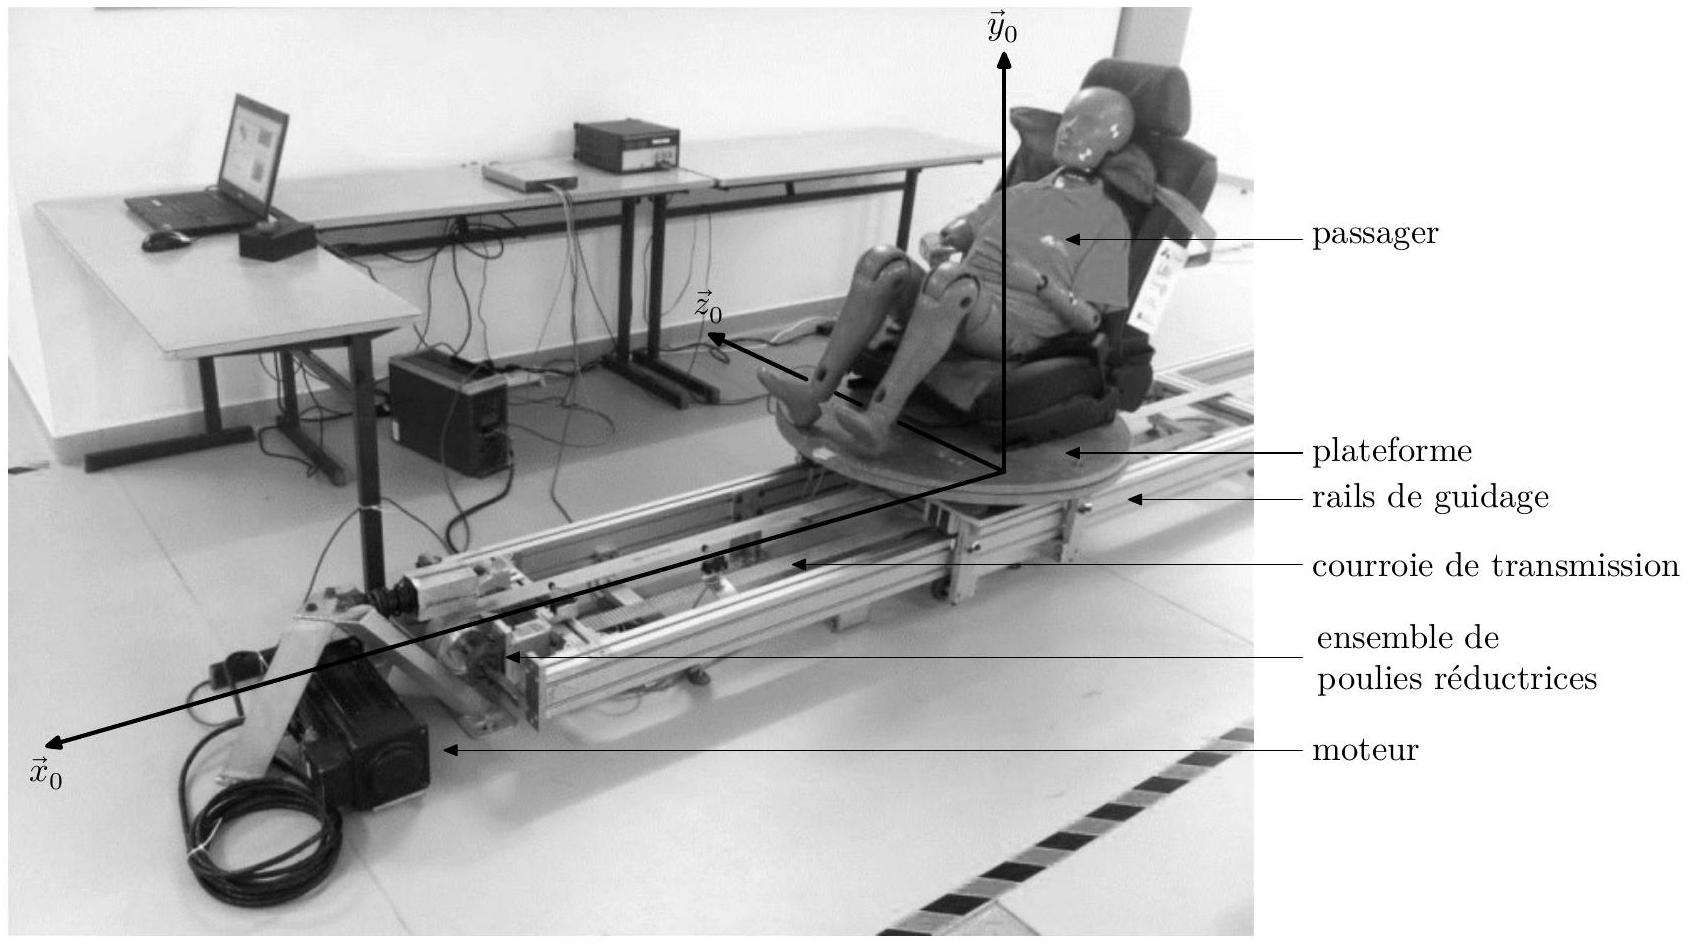
\includegraphics[width=.7\textwidth]{2025_07_06_ec63d2f3afc18cdeeb83g-10(1)}

%Figure 13 
\caption{\label{ccs_mp_2022_fig_13}Prototype du Sled (ou dispositif expérimental) à $0,3 g$}
\end{figure}
\fi

%IV.A - 
\subsection{Validation du choix de la motorisation effectué par le bureau d'études \label{ccs_mp_2022_sec_4A}}

\ifprof
\else
\begin{obj}
Dans un premier temps, il s'agit de valider le choix du moteur électrique retenu par les ingénieurs pour motoriser le prototype du Sled et répondre aux exigences.
\end{obj}

\subsubsection*{Hypothèses d'étude}
Compte tenu des dimensions du Sled définies lors du prédimensionnement, la chaine de transmission de puissance du moteur à l'ensemble mobile $S$ a été conçue et réalisée avec un système de poulies et de courroies comme représenté sur la figure \ref{ccs_mp_2022_fig_14}.

\begin{figure}[!h]
\centering
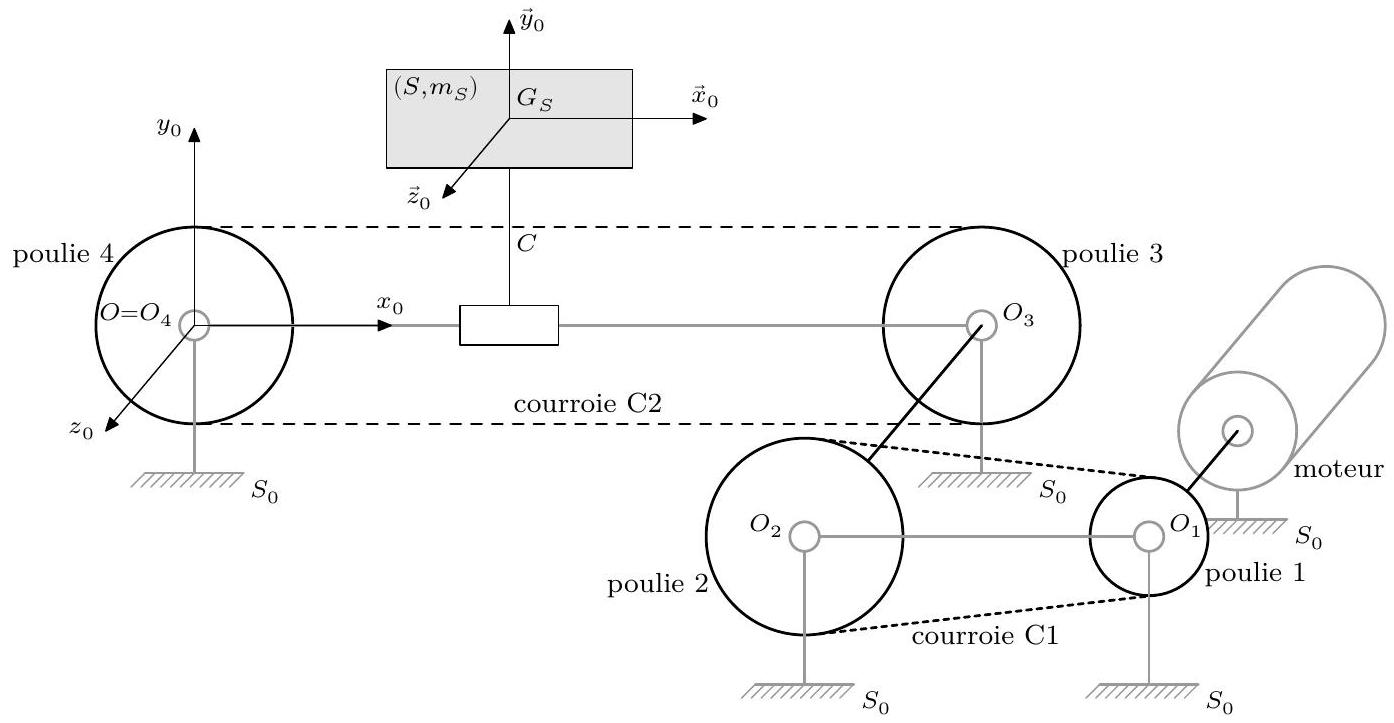
\includegraphics[width=.7\textwidth]{2025_07_06_ec63d2f3afc18cdeeb83g-10}

%Figure 14 
\caption{\label{ccs_mp_2022_fig_14}Modélisation cinématique de la chaine de transmission de puissance du prototype du Sled}
\end{figure}

Les poulies 1, 2 et la courroie C1 réalisent une adaptation de la vitesse de rotation en sortie du moteur électrique. Les poulies 3, 4 et la courroie C2 participent à la transformation de mouvement de rotation des poulies en mouvement de translation de l'ensemble mobile $S$.\\
Sur le prototype du Sled, le rendement global de la chaine de transmission de puissance prenant en compte tous les frottements (sec et fluide) est estimé à $\eta=55 \%$. La puissance totale ainsi perdue, notée $P_{\text {frottement }}$, s'exprime en fonction de la puissance fournie par le moteur : $P_{\text {frottement }}=(1-\eta) P_{\text {stator } \rightarrow \text { rotor } / S_{0}}$.

\subsubsection*{Notations et données}
\begin{itemize}
  \item $m_{S}$, masse de l'ensemble mobile $S=\{$ volontaire + siège + plateforme + capteurs $\}$.
  \item $t$, le temps, exprimé en secondes.
  \item $\vec{V}_{\left(G_{S}, S / S_{0}\right)}=v(t) \vec{x}_{0}$, la vitesse de déplacement du centre de gravité $G_{S}$ de l'ensemble mobile $S$ par rapport au bâti $S_{0}$.
  \item $J_{P_{1}}$, le moment d'inertie du sous-ensemble $P_{1}=\{$ poulie $1+$ rotor moteur $\}$ autour de son axe de rotation $\left(O_{1}, \vec{z}_{0}\right)$.
  \item $\vec{\Omega}_{\left(P_{1} / S_{0}\right)}=\omega_{1}(t) \vec{z}_{0}$, la vitesse angulaire de rotation d'axe ( $O_{1}, \vec{z}_{0}$ ) du sous-ensemble $P_{1}$ par rapport au bâti $S_{0}$.
  \item $\vec{C}_{m}=C_{m}(t) \vec{z}_{0}$, le couple exercé par le stator, lié à $S_{0}$, sur le rotor du moteur d'axe ( $O_{1}, \vec{z}_{0}$ ), avec $C_{m \text { max }}=$ $32 \mathrm{~N} \cdot \mathrm{~m}$ (donnée constructeur).
  \item $J_{P_{2}}$, le moment d'inertie équivalent du sous-ensemble $P_{2}=\{$ poulie $2+$ arbre de transmission + poulie $3+$ poulie $4+$ courroie C 2$\}$, rapporté à l'axe de rotation $\left(O_{2}, \vec{z}_{0}\right)$.
  \item $\vec{\Omega}_{\left(P_{2} / S_{0}\right)}=\omega_{2}(t) \vec{z}_{0}$, la vitesse angulaire de rotation de ce sous-ensemble $P_{2}$ par rapport au bâti $S_{0}$ autour de l'axe de rotation ( $O_{2}, \vec{z}_{0}$ ).
  \item $D_{2}=D_{3}=D_{4}=100 \mathrm{~mm}$, les diamètres des poulies 2,3 et 4 .
  \item $D_{1}=35 \mathrm{~mm}$, le diamètre de la poulie 1 .
  \item La masse et le moment d'inertie de la courroie C 1 sont négligés.
\end{itemize}
\fi

%Q 36. 
\question{\label{ccs_mp_2022_sec_q_36}Déterminer le rapport $k=\frac{\omega_{1}(t)}{\omega_{2}(t)}$.}
\ifprof
\begin{corrige}
$ k = \dfrac{\omega_1(t)}{\omega_2(t)} = \dfrac{D_2}{D_1}$ (en considérant une vitesse de glissement nulle entre la courroie et les poulies $1$ et $2$).
A.N. $ k = \dfrac{100}{35} \simeq 2.86$

C'est le rapport de transmission entre la poulie $1$ (en entrée) et la poulie $2$ (en sortie).
\end{corrige}
\else
\fi

%Q 37. 
\question{\label{ccs_mp_2022_sec_q_37}Déterminer $v(t)$ en fonction de $\omega_{1}(t)$ et d'un paramètre géométrique. Préciser les hypothèses nécessaires à la détermination de $k$ et de la relation entre $v(t)$ et $\omega_{1}(t)$.}
\ifprof
\begin{corrige}
$v(t) = \overrightarrow{V}_{G_S, S/S_0} \cdot \vec x_0$, or $\overrightarrow{V}_{G_S, S/S_0} = \overrightarrow{V}_{C, S/S_0} = \overrightarrow{V}_{C, C2/S_0} = \overrightarrow{V}_{I, C2/S_0} = \overrightarrow{V}_{I, \text{poulie } 3/S_0}$ (en considérant une vitesse de glissement nulle entre la poulie $3$ et la courroie C2).\\

Avec $I$ le point de contact entre la courroie C2 et la poulie $3$.

$\overrightarrow{V}_{I, \text{poulie } 3 /S_0} = \overrightarrow{V}_{O_3, \text{poulie } 3/S_0} + \overrightarrow{IO_3} \wedge \overrightarrow{\Omega}_{(P_3/S_0)}$

Or $\overrightarrow{\Omega}_{(P_3/S_0)} = \overrightarrow{\Omega}_{(P_2/S_0)} = \omega_2(t) \vec z_0$ \qquad car $\overrightarrow{\Omega}_{(P_3/P_2)} = \overrightarrow 0$

$\overrightarrow{V}_{I, \text{poulie } 3 /S_0} = \overrightarrow 0 + (-\dfrac{D_3}{2} \vec y_0) \wedge \omega_2(t) \vec z_0 = -\dfrac{D_3}{2} \omega_2(t) \vec x_0$, soit d'après la question 36 :
$ v(t) = - \dfrac{D_3 \, \omega_1(t)}{2 \, k}$.
\end{corrige}
\else
\fi


%Q 38. 
\question{\label{ccs_mp_2022_sec_q_38}En fonction de $\omega_{1}(t)$, exprimer l'énergie cinétique dans leur mouvement par rapport à $R_{0}\left(O, \vec{x}_{0}, \vec{y}_{0}, \vec{z}_{0}\right)$, repère supposé galiléen attaché à $S_{0}$, de}


\begin{itemize}
  \item la classe d'équivalence du sous-ensemble noté $P_{1}: E_{c}\left(P_{1} / S_{0}\right)$;
  \item la classe d'équivalence du sous-ensemble noté $P_{2}: E_{c}\left(P_{2} / S_{0}\right)$;
  \item la classe d'équivalence de l'ensemble mobile $S: E_{c}\left(S / S_{0}\right)$.
\end{itemize}

\ifprof
\begin{corrige}
\begin{itemize}
\item $E_c(P_1/S_0) = \dfrac{1}{2} J_{P_1} \omega_1(t)^2$ ;
\item $E_c(P_2/S_0) = \dfrac{1}{2} J_{P_2} \omega_2(t)^2 = \dfrac{1}{2} J_{P_2} \dfrac{\omega_1(t)^2}{k^2} $ ;
\item $E_c(S/S_0) = \dfrac{1}{2} m_S v(t)^2 = \dfrac{1}{2} m_S  \dfrac{D_3^2 \, \omega_1(t)^2}{4 \, k^2}$.
\end{itemize}
\end{corrige}
\else
\fi

%Q39
\question{\label{ccs_mp_2022_sec_q_39}Exprimer le moment d'inertie équivalent rapporté à l'axe moteur ( $O_{1}, \vec{z}_{0}$ ), noté $J_{\text {eq }}$, de la chaine de transmission de puissance composée des sous-ensembles $P_{1}, P_{2}$ et de l'ensemble mobile $S$, en fonction de $k, D_{1}$ et des différentes données inertielles propres à chaque classe d'équivalence.}
\ifprof
\begin{corrige}
$\begin{array}{ll}
E_c(\{P_1+P_2+S\}/S_0) &= \dfrac{1}{2} \left(  J_{P_1} + \dfrac{J_{P_2}}{k^2} + \dfrac{m_S D_3^2}{4 k^2}\right) \omega_1(t)^2 \\
&= \dfrac{1}{2} J_\text{eq} \omega_1(t)^2 \\
\end{array}$

Le rapport de transmission nous permet également d'écrire : $D_3 = D_2 = k \times D_1$

Finalement, on a : $ J_\text{eq} = J_{P_1} + \dfrac{J_{P_2}}{k^2} + m_S D_1^2$.
\end{corrige}
\else
\fi
%Q40
\question{\label{ccs_mp_2022_sec_q_40}Déterminer le couple $C_{m}(t)$. Il est attendu de préciser le système isolé, de détailler l'inventaire des différentes puissances intérieures et extérieures mises en jeu en les distinguant clairement, d'indiquer également les puissances qui sont nulles, en donnant une justification, et de donner l'expression du théorème utilisé.}
\ifprof
\begin{corrige}
On isole le système : \{ $P_1 + P_2 + S$ \}

Le bilan des puissances internes et externes est :
\begin{itemize}
\item $P_\text{externe} = P_\text{stator $\to$ rotor $/S_0$} = P_m = C_m \times \omega_1(t)$ ;
\item $P_\text{interne} = -P_\text{frottement} = -(1 - \eta) P_m$.\\
\end{itemize}

D'après le théorème de l'énergie cinétique (ou théorème de l'énergie puissance) appliqué au système isolé (et à l'aide de la question 39), on obtient la relation finale :

$ \dfrac{\text{d} E_c(P_1+P_2+S/S_0)}{\text{d}t} = P_\text{externe} + P_\text{interne}$
$ \Rightarrow  J_\text{eq} \dot\omega_1(t) \omega_1(t) = P_m  - (1 - \eta) P_m$
$ \Rightarrow  J_\text{eq} \dot\omega_1(t) {\omega_1(t)} = \eta C_m(t) \times {\omega_1(t)}$
$ \Rightarrow   C_m(t) = \dfrac{J_\text{eq}}{\eta} \dfrac{\text{d}\omega_1(t)}{\text{d}t}$.

\end{corrige}
\else
\fi

%Q 41. 
\question{\label{ccs_mp_2022_sec_q_41}Mettre $C_{m}(t)$ sous la forme $C_{m}(t)=\alpha \frac{\mathrm{d} v(t)}{\mathrm{d} t}$ en précisant l'expression de $\alpha$ en fonction de $J_{\text {eq }}, D_{1}$ et de $\eta$.\\
La suite du questionnement sera effectuée avec la valeur numérique $J_{\text {eq }}=0,064 \mathrm{~kg} \cdot \mathrm{~m}^{2}$.}
\ifprof
\begin{corrige}
D'après la question 37, on a : $\omega_1(t) = -\dfrac{2 \, k \, v(t)}{D_3} = -\dfrac{2 \, {k} \, v(t)}{{k} \, D_1} = -\dfrac{2 \, v(t)}{D_1} $, d'où :$ C_m(t) = - \dfrac{2 \, J_\text{eq}}{\eta \, D_1} \dfrac{\text{d}v(t)}{\text{d}t}$.
\end{corrige}
\else
\fi

%Q 42. 
\question{\label{ccs_mp_2022_sec_q_42}Tracer sur la copie, l'évolution du couple moteur en fonction du temps, correspondant au graphe de vitesse donné en figure \ref{ccs_mp_2022_fig_15}. Préciser les valeurs caractéristiques.}
\ifprof
\begin{corrige}
%\begin{center}
%	\begin{tikzpicture}
%	\coordinate (O) at (0,0);
%	\def \myxf{10}
%	\def \myyf{3.2}
%	\def \myU{2}
%	\def \mytz{5}
%		\draw [->,>=latex] ($(O)+(-.5,0)$) -- node[pos=1,anchor=west] {$t$ [s]} ($(O)+(\myxf+1,0)$) ;
%		\draw [->,>=latex] ($(O)+(0,-3.2)$) -- node[pos=1,anchor=south, blue] {$C_m(t)$}  ($(O)+(0,\myyf)$) ;
%		\draw[blue, thick] ($(O)+(0,-2)$) -- (\mytz,-2) -- (\mytz,\myU) -- (\myxf-.5,\myU); 
%		\draw[black] (0,-.1) -- node[pos=0,anchor=north east] {$0$} (0,.1);
%		\draw[black] (\mytz,-.1) -- node[pos=0,anchor=north east] {$1$} (\mytz,.1);
%		\draw[black] (\myxf,-.1) -- node[pos=0,anchor=north east] {$2$} (\myxf,.1);
%		\draw[black] (-.1,\myU) -- node[pos=0,anchor=east] {$\dfrac{2 \, J_\text{eq} \times 0.3 g}{\eta D_1}$} (.1,\myU);
%		\draw[black] (-.1,-\myU) -- node[pos=0,anchor=east] {$-\dfrac{2 \, J_\text{eq} \times 0.3 g}{\eta D_1}$} (.1,-\myU);
%
%	\end{tikzpicture}
%\end{center}

\end{corrige}
\else
\fi


\ifprof
\else


\begin{figure}[!h]
\centering
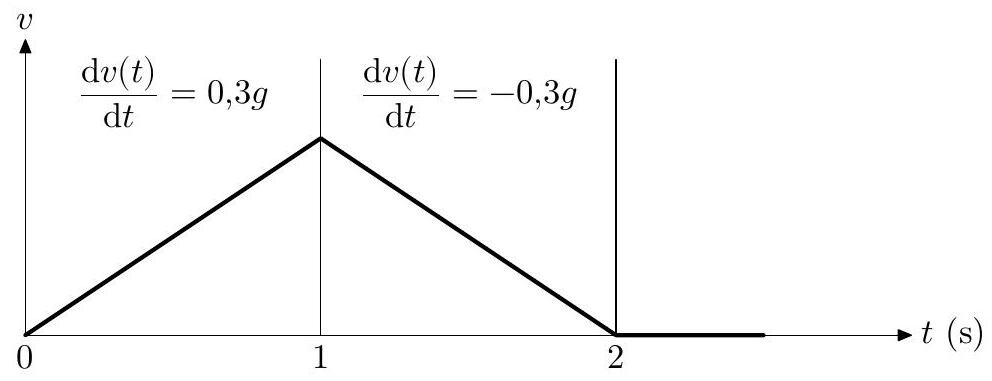
\includegraphics[width=.7\textwidth]{2025_07_06_ec63d2f3afc18cdeeb83g-11}

%Figure 15 
\caption{\label{ccs_mp_2022_fig_15}Évolution de la vitesse de l'ensemble mobile}
\end{figure}
\fi

%Q 43. 
\question{\label{ccs_mp_2022_sec_q_43}Conclure quant au choix de moteur effectué par les ingénieurs du bureau d'études sur ce critère de couple moteur.}
\ifprof
\begin{corrige}
Le moteur choisi par les ingénieurs permet de délivrer un couple maximal de : $C_{m\text{max}} = 32$ N.m.

Le couple moteur a un couple maximal d'après la \textsc{Figure} \ref{fig:sled15} de $C_m = \dfrac{2 \, J_\text{eq} \times 0.3 g}{\eta D_1}$.

A.N. :$ C_m = \dfrac{2 \times 0.064 \times 0.3 \times 9.81}{0.55 \times 35 \times 10^{-3}} \simeq 19.6 \text{ N.m}$.

Le moteur a donc été dimensionné avec un coefficient de sécurité de $1.5$. Le moteur choisi par les ingénieur peut fournir le couple nécessaire à l'évolution de la vitesse de l'ensemble mobile.
\end{corrige}
\else
\fi


%IV.B - 
\subsection{Analyse des essais réalisés sur le prototype du Sled pour les conditions $\pm 0,3 g$}

\begin{obj}
L'objectif est de vérifier si les performances du prototype ainsi motorisé sont conformes aux exigences (figure \ref{ccs_mp_2022_fig_A}).
\end{obj}
\ifprof
\else


Trois tests expérimentaux, avec une masse embarquée de 80 kg représentative d'un volontaire, ont été réalisés sur le prototype du Sled (figure \ref{ccs_mp_2022_fig_16}). La figure \ref{ccs_mp_2022_fig_17} représente les écarts relatifs entre les essais respectifs.\\


\begin{figure}[!h]
\centering
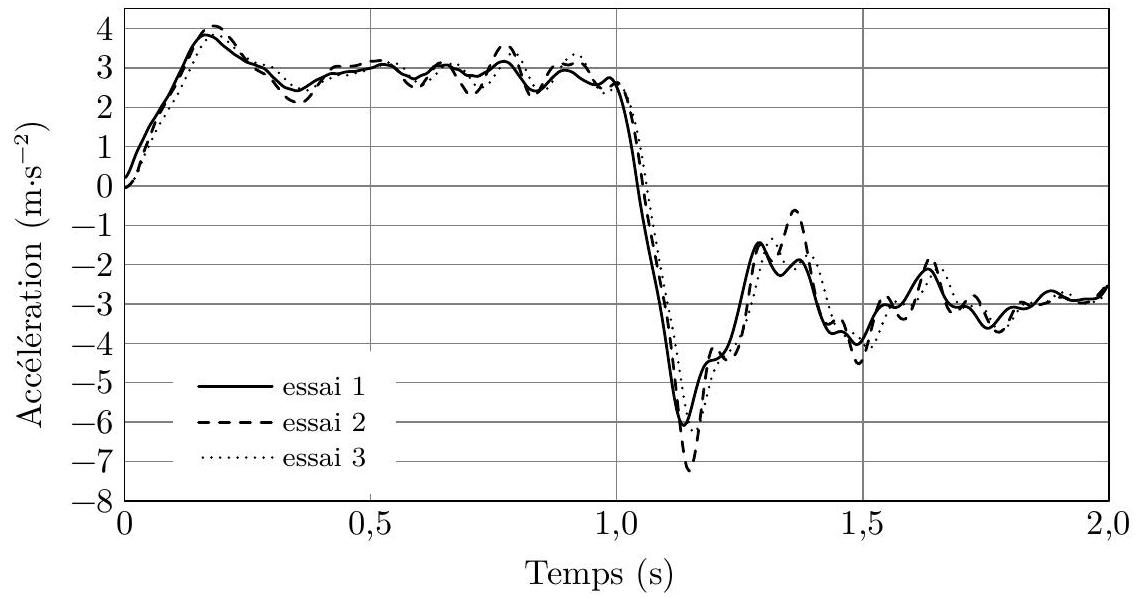
\includegraphics[width=\textwidth]{2025_07_06_ec63d2f3afc18cdeeb83g-12}
%Figure 16 
\caption{\label{ccs_mp_2022_fig_16}Résultats temporels des 3 essais}
\end{figure}


\begin{figure}[!h]
\centering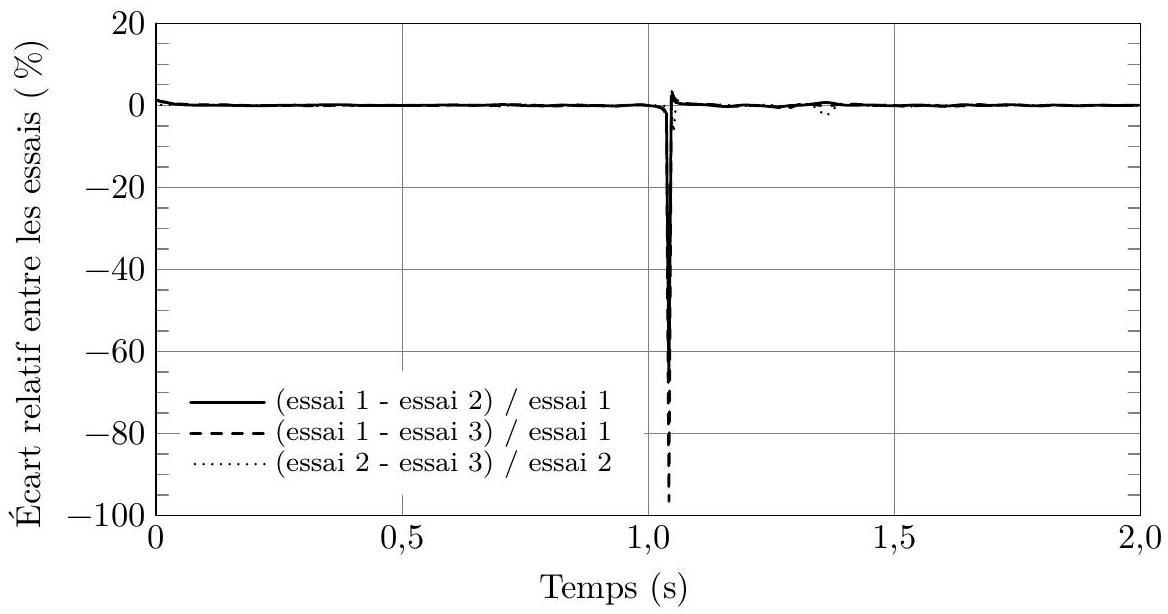
\includegraphics[width=\textwidth]{2025_07_06_ec63d2f3afc18cdeeb83g-12(1)}
%Figure 17 
\caption{\label{ccs_mp_2022_fig_17}Écarts expérimentaux relatifs entre les 3 essais}
\end{figure}



La durée totale de l'essai, accélération puis décélération, est de 2 secondes.\\
Prioritairement, les ingénieurs du bureau d'études veulent garantir :

\begin{itemize}
  \item la stabilité du système asservi, exigence Id = 1.1.1.1 ;
  \item la robustesse, exigence $\mathrm{Id}=1.1 .1 .3$.
\end{itemize}

Pour s'affranchir de la discontinuité en accélération, les ingénieurs du bureau d'études se limitent à l'étude en régime établi en négligeant la phase de transition entre l'accélération et la décélération autour de 1 seconde.
\fi

%Q 44. 
\question{\label{ccs_mp_2022_sec_q_44}Reproduire sur un croquis une des courbes de la figure \ref{ccs_mp_2022_fig_16} pour l'intervalle de temps $[0 \mathrm{~s}, 1 \mathrm{~s}]$. En s'appuyant sur ce croquis et une analyse chiffrée, indiquer si l'exigence $\mathrm{Id}=1.1 .1 .1 .2$ est atteinte.}
\ifprof
\begin{corrige}
%\begin{center}
%	\begin{tikzpicture}
%	\coordinate (O) at (0,0);
%	\def \myomega{2}
%	\def \myxf{10}
%	\def \myyf{4.5}
%	\def \myK{2.94}
%	\def \mytz{0}
%	\def\myT{2}
%	\def\myksii{.24}
%	\def\l{.2}
%	\def\mysmax{\myK*(1+exp(-pi*\myksii/sqrt(1-\myksii^2)))}
%	\def\myTp{2*pi/(\myomega*sqrt(1-\myksii^2))}
%	\def\tmax{\mytz + pi/(\myomega*sqrt(1-\myksii^2))}
%		\draw [->,>=latex] ($(O)+(-.5,0)$) -- node[pos=1,anchor=west] {$t$ [s]} ($(O)+(\myxf+.5,0)$) ;
%		\draw [->,>=latex] ($(O)+(0,-.5)$) -- node[pos=1,anchor=south, blue] {$\ddot x \text{ [m.s$^{-2}$]}$} ($(O)+(0,\myyf)$) ;
%		\draw[black] (\mytz,-.1) -- node[pos=0,anchor=north east] {$0$} (\mytz,.1);
%		\draw[black] (-.1,\myK) -- node[pos=0,anchor=east] {$2.94$} (.1,\myK);
%		\draw[black, dashed] (0,\myK) -- (\myxf-.5,\myK);
%		\draw[black] (-.1,{\mysmax}) -- node[pos=0,anchor=east] {$4$} (.1,{\mysmax});
%		\draw[black,dashed] (0,{\mysmax}) -- (4,{\mysmax}) ;
%	\draw[blue, thick, domain=\mytz:\myxf-.5, samples=150] 	plot	
%(\x,{\myK*(1-((exp(-\myomega*\myksii*(\x-\mytz))/sqrt(1-\myksii^2))*sin((180/pi)*\myomega*sqrt(1-\myksii^2)*(\x-\mytz)+atan(sqrt(1-\myksii^2)/\myksii))))});
%		\draw[<->,>=latex] ({\tmax},1) -- node[anchor=north] {$T_n$} ++  ({\myTp},0);
%		\draw[dashed] ({\tmax},1) --++ (0,3);
%		\draw[dashed] ({\tmax+\myTp},1) --++ (0,2.5);
%		\draw[black] (\myxf,-.1) -- node[pos=0,anchor=north east] {$1$} (\myxf,.1);
%	\end{tikzpicture}
%\end{center}

On a alors un dépassement de $\dfrac{4 - 2.94}{2.94} \simeq 0.36 \quad \text{soit 36\%} > 20\%$. L'exigence \texttt{Id : 1.1.1.1.2} n'est donc pas respectée.
\end{corrige}
\else
\fi

%Q 45. 
\question{\label{ccs_mp_2022_sec_q_45}À partir de la figure \ref{ccs_mp_2022_fig_17}, montrer de façon chiffrée que l'exigence Id $=1.1 .1 .3 .1$ est atteinte pour les conditions d'essais et d'interprétation fixées.}
\ifprof
\begin{corrige}
On peut observer en \textsc{Figure} \ref{fig:sled16} après une seconde, que l'écart relatif entre deux essais dépasse les $5\%$. L'exigence \texttt{Id : 1.1.1.3.1} n'est donc pas respectée.
\end{corrige}
\else
\fi

%IV.C - 
\subsection{Évolutions du modèle multiphysique \label{ccs_mp_2022_sec_4C}}
\begin{obj}
%\section*{Objectif}
L'objectif recherché par les ingénieurs du bureau d'études est à présent d'affiner les performances du modèle multiphysique et du dispositif expérimental (ou prototype) du Sled $0,3 g$.
\end{obj}

\ifprof
\else

La confrontation des performances expérimentales, avec celles obtenues en simulation avec le modèle $\mathrm{n}^{\circ} 1$ (figure \ref{ccs_mp_2022_fig_20}), permet d'affirmer que le modèle $n^{\circ} 1$ n'est pas totalement représentatif du comportement réel du prototype du Sled. Un modèle multiphysique $\mathrm{n}^{\circ} 2$ (figure \ref{ccs_mp_2022_fig_21}) est développé. Il comporte désormais à la fois
la correction PI précédemment définie, mais aussi une prise en compte plus réaliste de la partie mécanique précédemment décrite.

Le résultat de la simulation de ce modèle $\mathrm{n}^{\circ} 2$ (figure \ref{ccs_mp_2022_fig_21}) à une consigne d'accélération en échelon de $0,3 g$ est présenté sur la figure \ref{ccs_mp_2022_fig_18}. Le résultat expérimental du prototype du Sled est également représenté sur cette figure et peut ainsi être comparé. Le résultat de la simulation du modèle $\mathrm{n}^{\circ} 1$ avec correction proportionnelle intégrale y est également rappelé. Les trois courbes correspondent à une même masse embarquée de 80 kg .

\begin{figure}[!h]
\centering

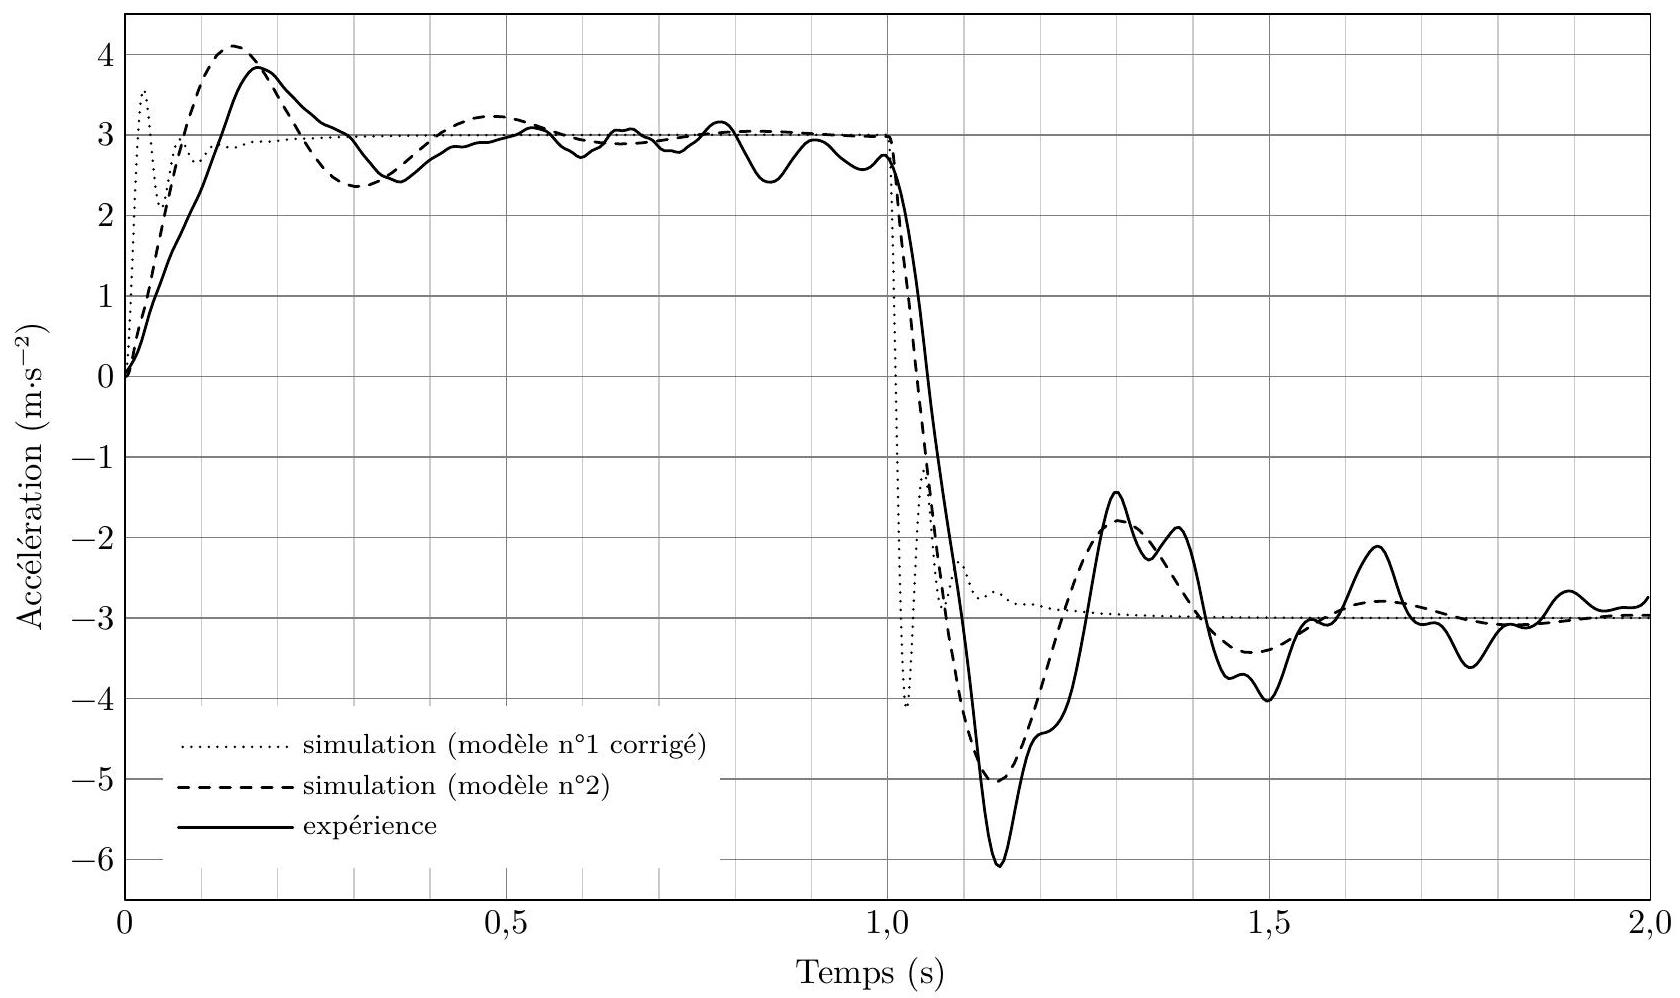
\includegraphics[width=\textwidth]{2025_07_06_ec63d2f3afc18cdeeb83g-13}

%Figure 18 
\caption{\label{ccs_mp_2022_fig_18}Comparaison des résultats expérimentaux sur le prototype du Sled avec ceux issus des deux simulations. }
Légende :

\begin{itemize}
  \item << expérience >>, résultats expérimentaux obtenus avec le Sled;
  \item << simulation (modèle $\mathrm{n}^{\circ} 2$ ) >>, le modèle $\mathrm{n}^{\circ} 2$ comportant la correction PI comme défini en figure \ref{ccs_mp_2022_fig_21} ;
  \item << simulation (modèle $\mathrm{n}^{\circ} 1$ corrigé) >>, modèle $\mathrm{n}^{\circ} 1$ défini en figure \ref{ccs_mp_2022_fig_20} avec ajout d'une correction PI définie à partir de la figure \ref{ccs_mp_2022_fig_10}.
\end{itemize}
\end{figure}


Il apparait que la courbe << simulation (modèle $\mathrm{n}^{\circ} 2$ ) >> est plus proche de la courbe << expérience >> que la courbe intitulée << simulation (modèle $\mathrm{n}^{\circ} 1$ corrigé) >>. Elle présente plus de dépassements et d'oscillations. Le second modèle présenté en figure \ref{ccs_mp_2022_fig_21} est donc plus proche de la réalité du prototype du Sled $0,3 g$ que le modèle multiphysique $\mathrm{n}^{\circ} 1$ (figure \ref{ccs_mp_2022_fig_20}) avec correction (figure \ref{ccs_mp_2022_fig_10}).

Dans cette comparaison, l'apport du modèle multiphysique $n^{\circ} 2$ se situe principalement sur l'ajout de la zone entourée d'un ovale en figure \ref{ccs_mp_2022_fig_21}.
\fi


%Q 46. 
\question{\label{ccs_mp_2022_sec_q_46}Préciser quel composant technologique du prototype du Sled est modélisé par la zone entourée d'un ovale en figure \ref{ccs_mp_2022_fig_21} et qui permet de diminuer l'écart entre le résultat de la «simulation (modèle $\mathrm{n}^{\circ} 2$ ) » et le comportement expérimental.}
\ifprof
\begin{corrige}
Le composant technologique modélisé par la zone entourée d'un ovale est la courroie C2.
\end{corrige}
\else
\fi
